
\chapter{Controle velocidade}


\section{Cálculo de velicidade do motor}

Como encoder possuí dois sinais de onda quadadra, de valores lógicos HIGH e LOW, e direção de rotação do motor pode ser definida pela diferença de fase 
É possível calcular a velocidade com base nas subidas da onda quadrada de uma fase, e o valor logico da outra fase no momento da subida.
Por exemplo,  observando a fase B, toda vez em que há uma subida, se o valor da fase A for alto, então incrementar +1 em um contador, se a fase A tiver valor baixo, então incrementar -1 no contador.
Quando o valor da fase A for alto, então o motor esta rodando em um sentido,  quando o valor  for baixo, então o motor esta rodando no sentido contrário.
Medindo o valor do contador por um $\Delta_{T}$, se resulta na quantidade de pulsos por segundo.
Para converter de pulsos por segundo para RPM, basta dividir pela resolução do motor+encoder,  que é de 1:34 do motor, e 11 pulsos por rotação do encoder, o que resulta em 374,
e multiplicar por 60 para ter o resultado em rotações por minuto.


\begin{tikzpicture}[node distance=2cm]

    \node (start) [startstop] {início loop};
    \node (pro1) [process, below of=start] {ENQUANTO DELTA T};
    
    \node (in1) [io, right of=pro1, xshift= 4cm] {QUANDO FASE B = SUBIDA};
    
    \node (dec1) [decision, below of=in1, yshift=-2cm] {SE FASE A = 1};
    \node (pro1a) [process, below of=dec1, yshift= -2cm] {INCREMENTAR CONTADOR em +1};
    \node (pro1b) [process, right of=dec1, xshift= 3cm] {INCREMENTAR CONTADOR em -1};
    
    
    \node (count) [process, below of=pro1, yshift= -9cm] {CONTADOR DIVIDO POR DELTA T};
    
    \draw [arrow] (start) -- (pro1);
    \draw [arrow] (pro1) -- node[anchor=north] {sim} (in1);
    \draw [arrow] (in1) -- (dec1);
    \draw [arrow] (dec1) -- node[anchor=east] {sim} (pro1a);
    \draw [arrow] (dec1) -- node[anchor=north] {não} (pro1b);
    
    \draw [arrow] (pro1) -- node[anchor=east] {não} (count);
    
\end{tikzpicture}
    


Na implementação dessa lógica no STM32, o desafio foi a definição do $\Delta_{T}$,
Se o $\Delta_{T}$ for muito pequeno, o resultados de pulsos por segundo pode tender ao infinito, gerando valores muito altos.
Na figura \ref{fig:medidas_altas} em laranja, esta o resultado do rpm considerando o $\Delta_{T}$ como o tempo entre os ciclos do micrcontrolador.
A outra opção, foi definir um $\Delta_{T}$ fixo, definindo uma frequencia de medição pré definida, e o resultado pode ser visto em azul na figura \ref{fig:medidas_altas}
Essa outra opção de $\Delta_{T}$ resultou em um sinal que tem uma componente em alta frequência com uma amplitude até consideral.
Analisando os dois sinai no dominio da frequêcia \ref{fig:frequencia_medidas_altas}, o espectro em frequência do sinal em laranja possui amplitudes muitos semelhante em todo espectro, mas o espectro do sinal em azul, fica bem claro que em altas frequencias é composto mais por ruidos
e as frequencia médias tem amplitude menor em relação as frequências baixas, o que torna mais fácil aplicar um filtro passa-baixa para reduzir as frenquências médias e altas.


\begin{figure}[h]
	\centering
	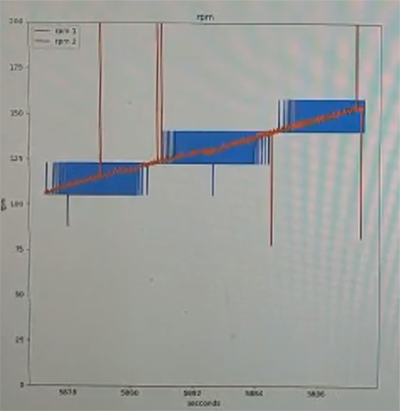
\includegraphics{figures/medidas_altas}
	\caption{Problemas com delta T muito pequeno}
	\label{fig:medidas_altas}
\end{figure}


A figura \ref{fig:passa_baixa_teste}, mostra um dos teste de filtro passa baixa, em o sinal em laranja ainda persiste esses valores tentendo ao infinito, devido a ampliture eles se tornam um pouco dificil de serem retirados.
Mas o sinal em azul acaba tendo um resultado melhor depois do filtro, muito semelhando ao sinal em laranja.
Com base nesse resultado, foi decidido seguir com o método em que o $\Delta_{T}$ é definido por uma frequência pré definida.

\begin{figure}[h]
	\centering
	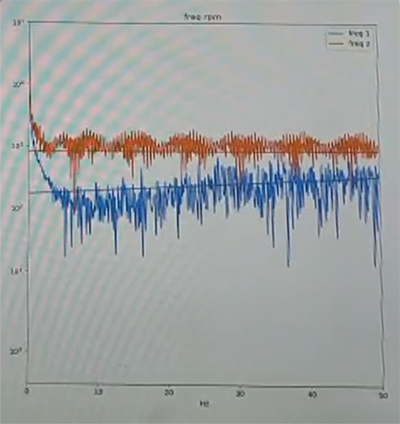
\includegraphics{figures/frequencia_medidas_altas}
	\caption{Frequências}
	\label{fig:frequencia_medidas_altas}
\end{figure}


\begin{figure}[h]
	\centering
	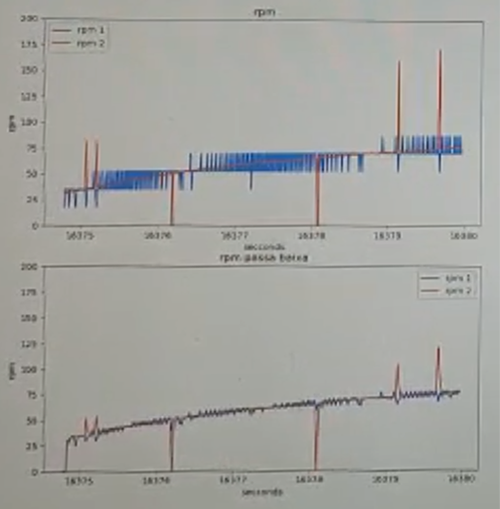
\includegraphics{figures/passa_baixa_teste}
	\caption{Passa baixa teste}
	\label{fig:passa_baixa_teste}
\end{figure}

Com o método definido, foi definido um $\Delta_{T}$ em 100hz eu um filtro passa baixa em 2hz
as seguintes imagens mostram o resultado do sinal original, filtrado via python e 
filtrado direto via microcontrolador, para cada motor ()\ref{fig:medidas_motor_1},  \ref{fig:medidas_motor_2} , \ref{fig:medidas_motor_3}).


\begin{figure}[h]
	\centering
	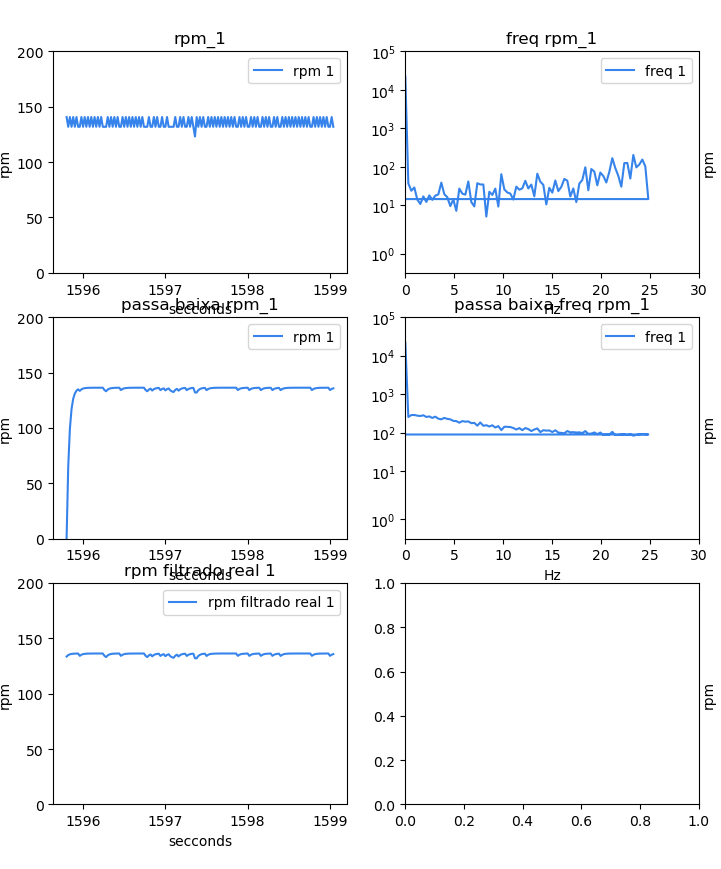
\includegraphics{figures/medidas_motor_1}
	\caption{Medidas Motor 1}
	\label{fig:medidas_motor_1}
\end{figure}

\begin{figure}[h]
	\centering
	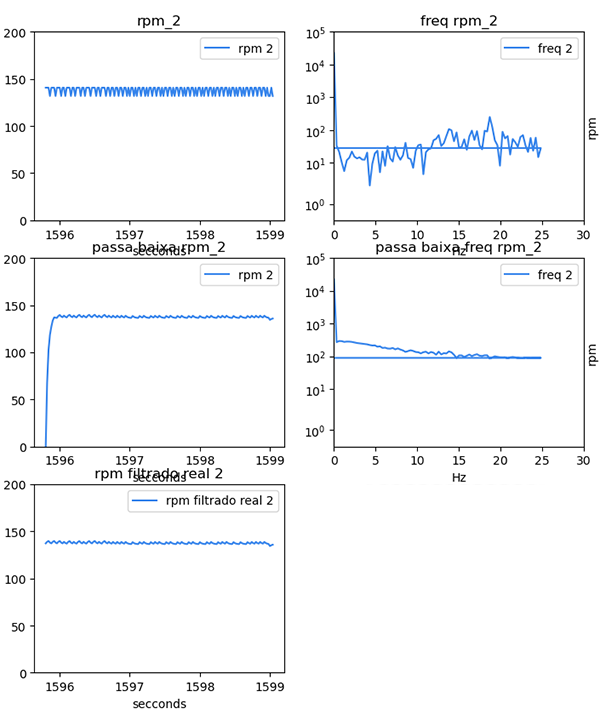
\includegraphics{figures/medidas_motor_2}
	\caption{Medidas Motor 2}
	\label{fig:medidas_motor_2}
\end{figure}


\begin{figure}[h]
	\centering
	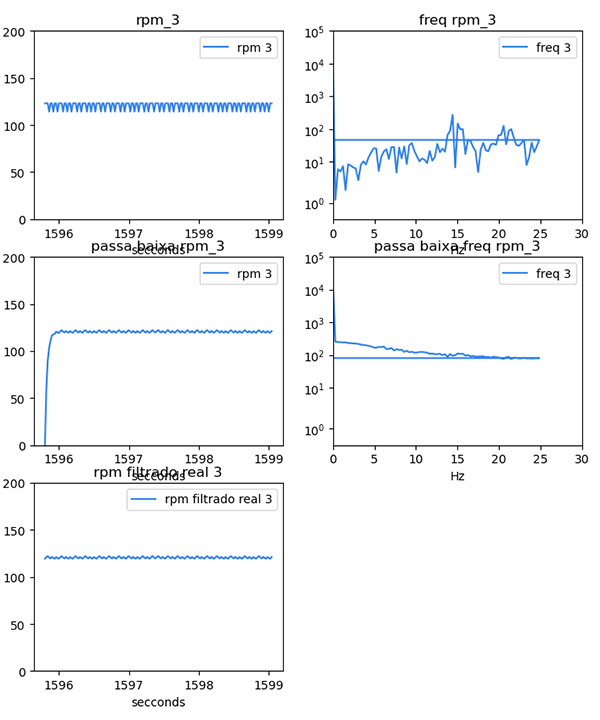
\includegraphics{figures/medidas_motor_3}
	\caption{Medidas Motor 3}
	\label{fig:medidas_motor_3}
\end{figure}